  {  \scriptsize
    \def\subBoxWidth{38cm}
    \def\subjectBoxWidth{80cm}
    \def\subjectRowHeight{52.5cm}
    \def\topRowHeightLeft{26.5cm}
    \def\topRowHeightRight{22.5cm}
    \def\bottomRowHeightLeft{12.5cm}
    \def\bottomRowHeightRight{16.5cm}
    \node[anchor=north west, boxStyle, text width=\subjectBoxWidth, anchor=north west, minimum height=\subjectRowHeight] (subjects) at ($(cmsBox.south west)+(0,-1.5)$){
    };
 %   \node[fancytitle, left=\titleOffset] at (subjects.north east) {Thesis subjects 2016-2017};

    \node[anchor=north,color=white, text width=70cm] at ($(subjects.north)+(0,-.5)$){
          \small
          The Ghent CMS team is involved in several analyses at CMS, which include supersymmetry searches, top quark physics, and searches for heavy sterile neutrinos.
          Master students are welcome to join in one of our analyses groups where they get the opportunity to explore the large amounts of new data.
          Under the daily supervision of our CMS team, you will acquire the necessary knowledge to identify particles, select the events of interest and to use big data analysis techniques.
          You get the opportunity to gain experience in an international collaboration, and present/discuss results at CERN.
    };
    
    \node[insideBoxStyle, text width=\subBoxWidth, anchor=north east,minimum height=\topRowHeightLeft] (top) at ($(subjects.north)+(-1,-8)$){
       {\tiny \\} \hspace{0.5cm}
       \begin{minipage}{20cm}
       {\tiny
       The heaviest particle in the Standard Model is the top quark. 
       As such, its properties are very sensitive to the existence of new physics beyond the SM.
       If we study top-quark production in processes where they appear together with electroweak bosons, 
       we get an excellent handle on the SM electroweak sector, as well as on top quark properties. 
       These properties can be measured using a number of production modes and decay channels. 
       We propose theses on measuring the rates of single top quark or top-quark pair production in association with $W$ and $Z$ bosons. 
       The production of a single top quark in combination with a $Z$ boson was discovered for the very first time last year by the Ghent CMS group,
       based on a partial Run II dataset. We propose a thesis project to help improve the existing analysis techniques in the context of 
       a new analysis that will use the full Run 2 dataset for this high-profile measurement.}
       \hspace{5mm}
         \begin{itemize}
     %     \color{white}
          \tiny
          \item Precision measurement of top quark pair production in association with $W$ and $Z$ bosons 
          \item Precision measurement of a single top-quark in association with a $Z$ boson
         \end{itemize}

       \end{minipage}
       \begin{minipage}{15cm}
           \hspace{5cm}    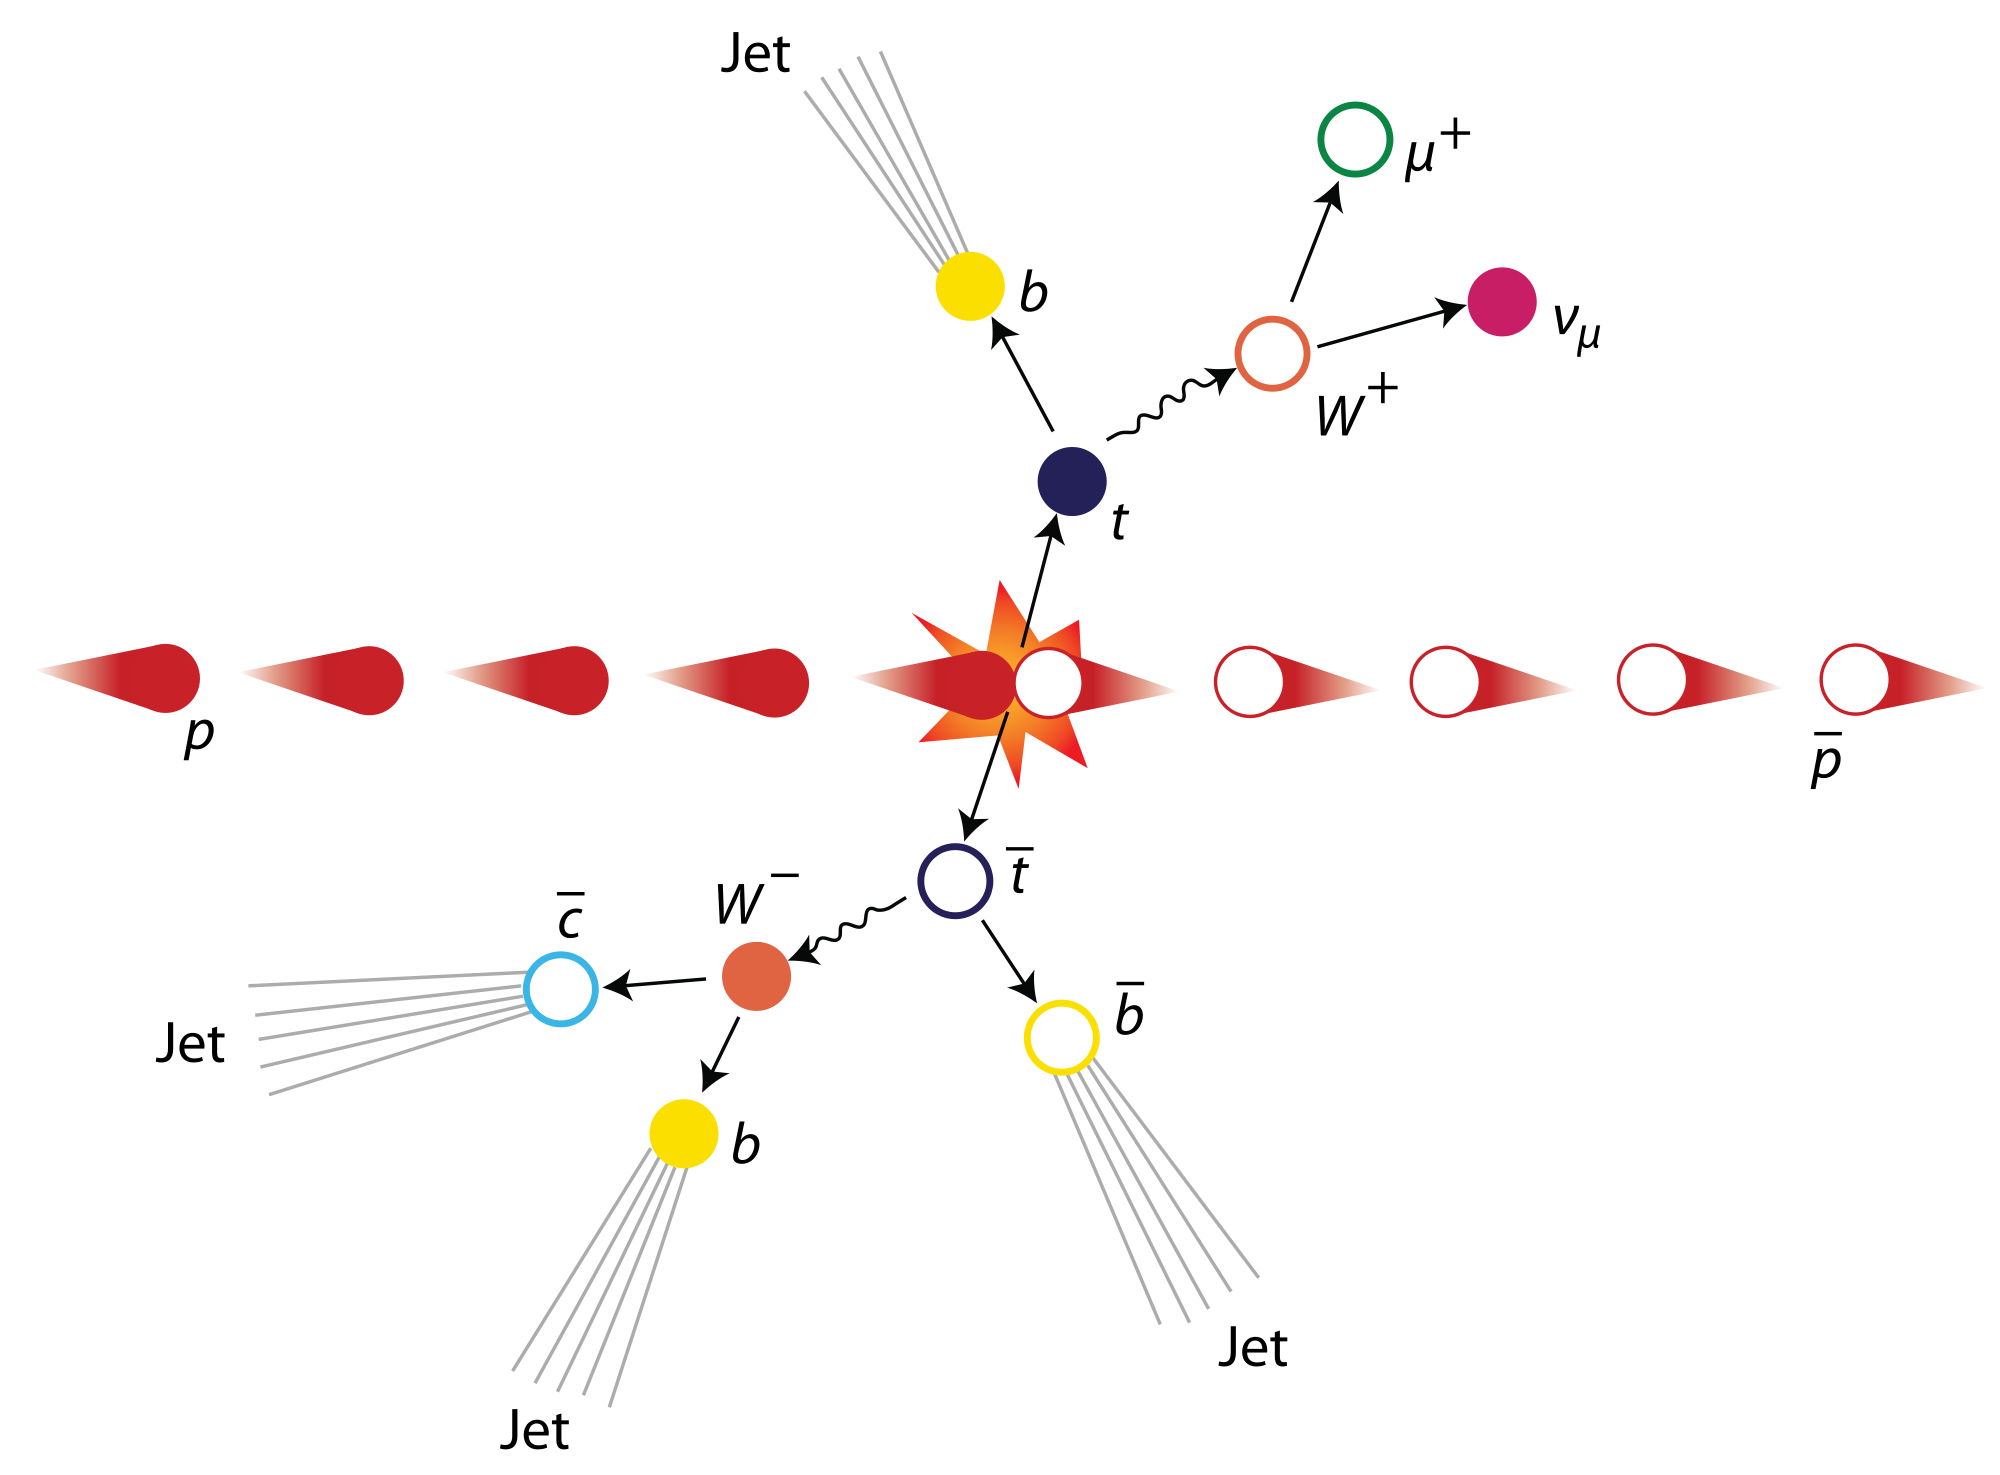
\includegraphics[width=9cm]{top.png}
           \vspace{-1cm} \\
           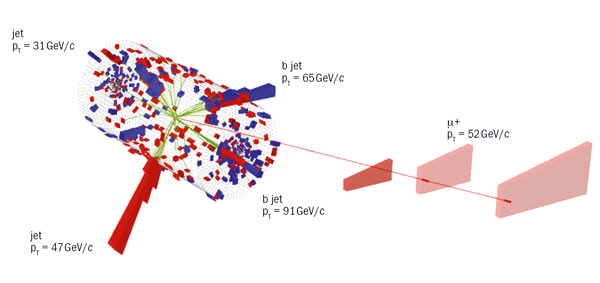
\includegraphics[width=15cm]{top2.png} 
       \end{minipage}
       \begin{minipage}{16cm}
         \begin{center}
         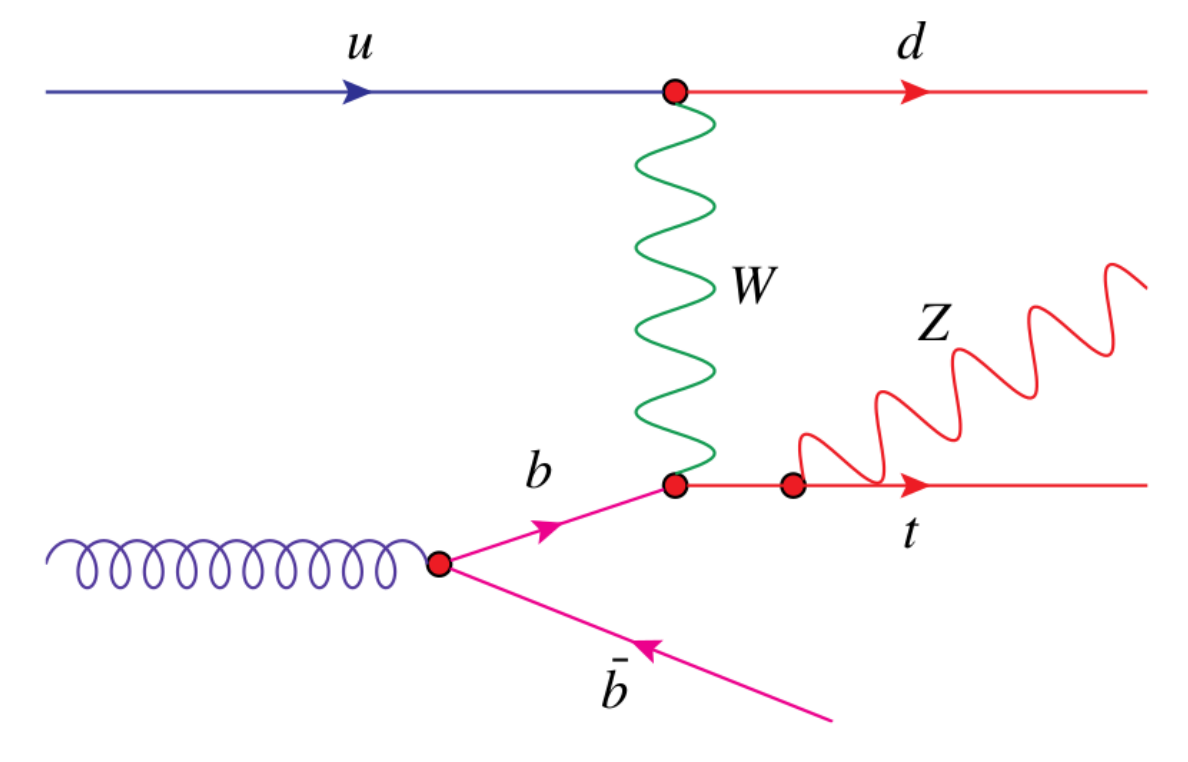
\includegraphics[width=0.9\textwidth]{tZq2.png} 
         \end{center}
       \end{minipage}
       \hspace{5mm}
       \begin{minipage}{20cm}
       \hspace{15mm}
         \begin{center}
         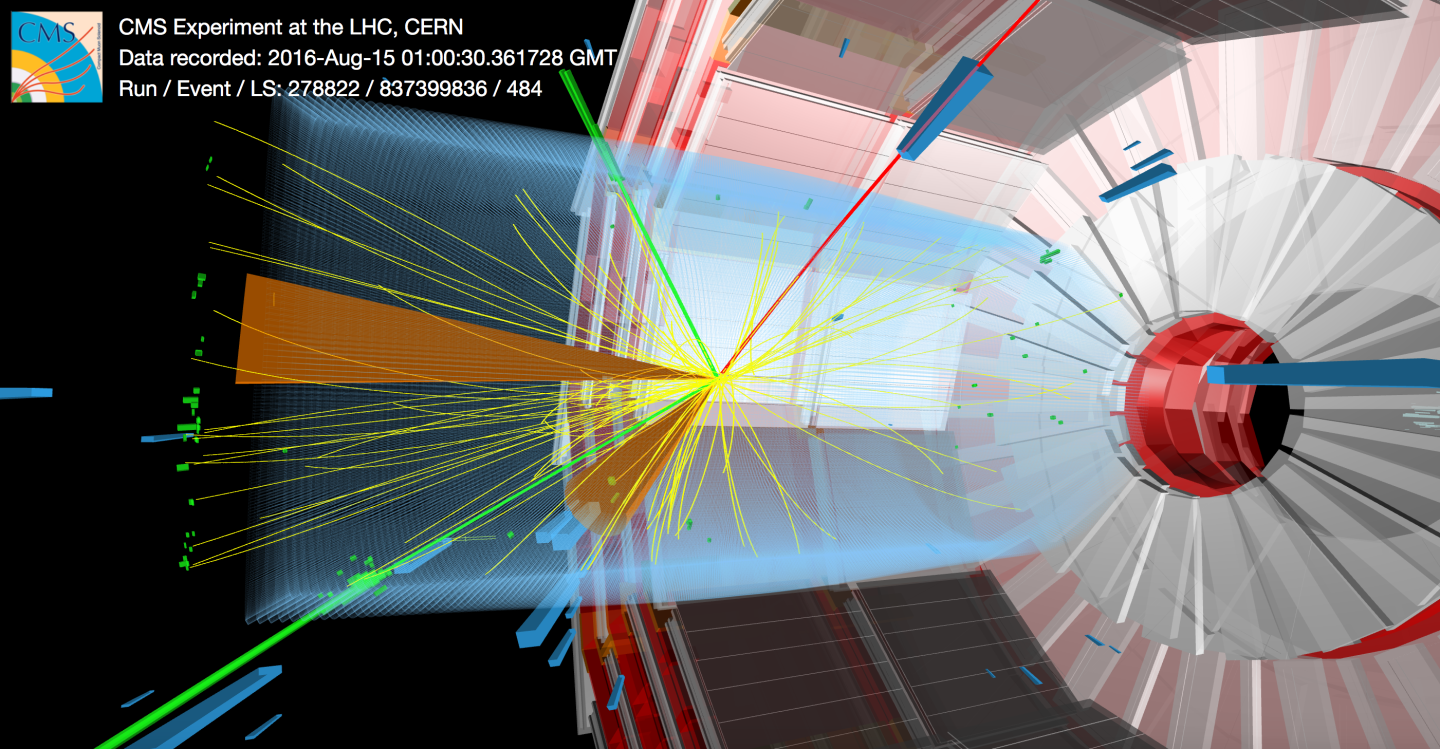
\includegraphics[width=0.9\textwidth]{tZq.png} 
         \end{center}
       \end{minipage}



    };
    \node[insideFancytitle, left=\insideTitleOffset] at ($(top.north east)+(0,0.5)$){\normalsize Precise measurements in top quark sector}; 
   
 
     \node[insideBoxStyle, text width=\subBoxWidth, anchor=north east,minimum height=\bottomRowHeightLeft] (nn) at ($(top.south east)+(0,-2.5)$){
       {\tiny \\} \hspace{0.5cm}
       {\tiny 
       \begin{minipage}{37cm}
         While searches for SUSY might be considered as dark matter searches, one can also look for direct production of other possible dark matter candidates, without involving a cascade decay of SUSY particles.
       \end{minipage}
       
       }
        \begin{figure}
                           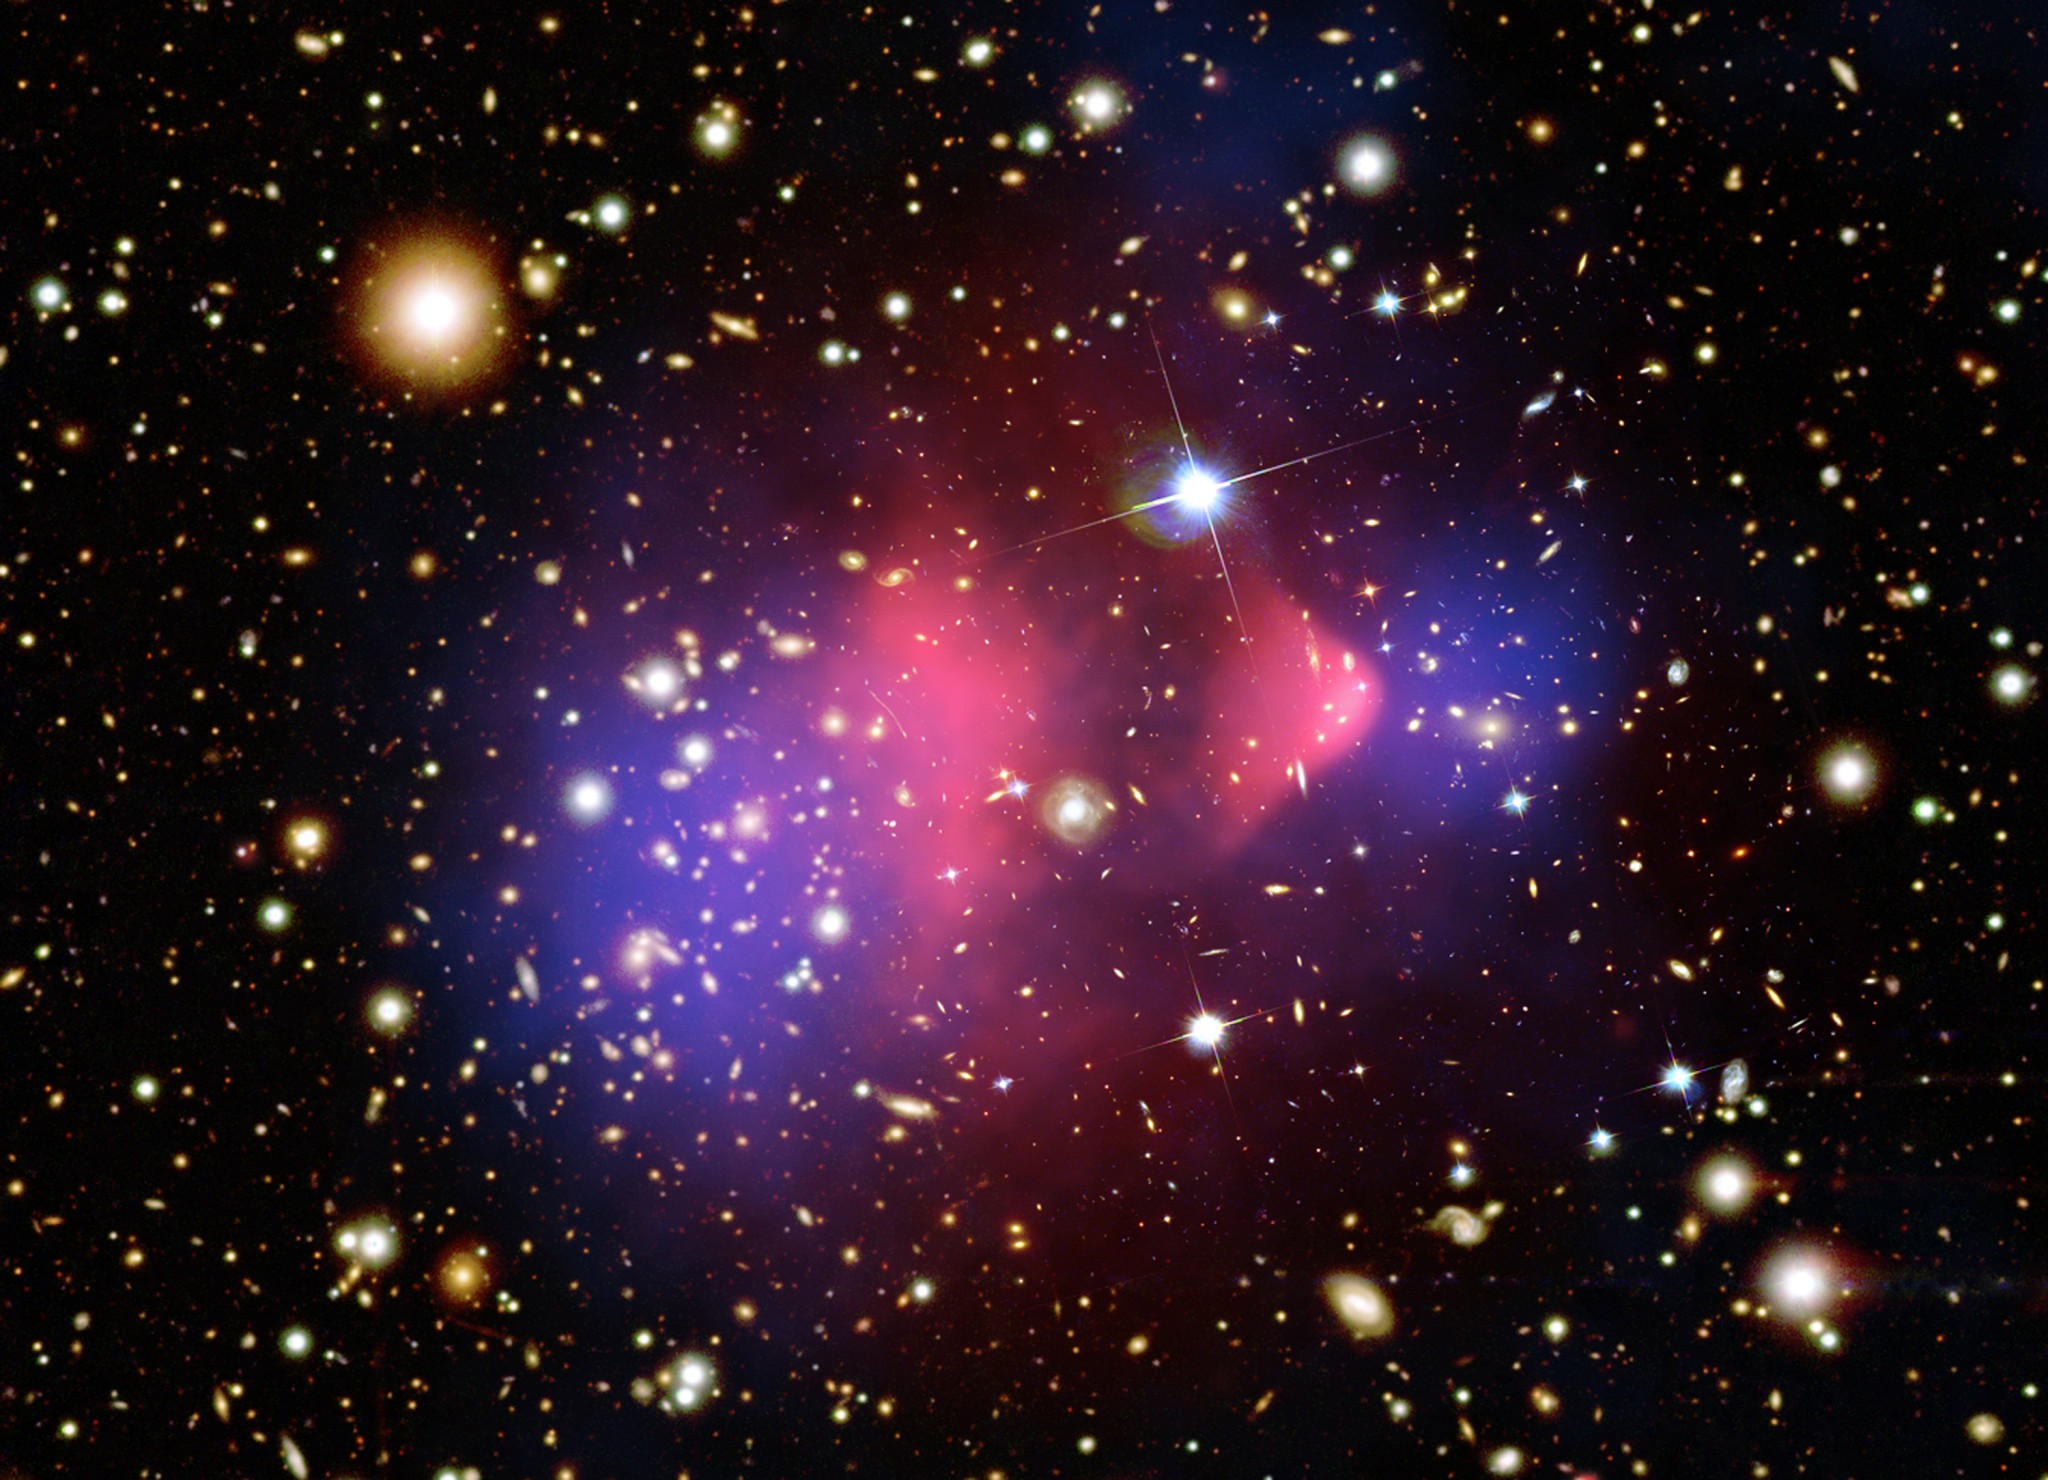
\includegraphics[height=7cm]{bc.jpg}
                           \hspace{3cm}
                           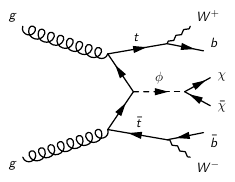
\includegraphics[height=7cm]{DMdiagram.png}
                           \hspace{3cm}
                           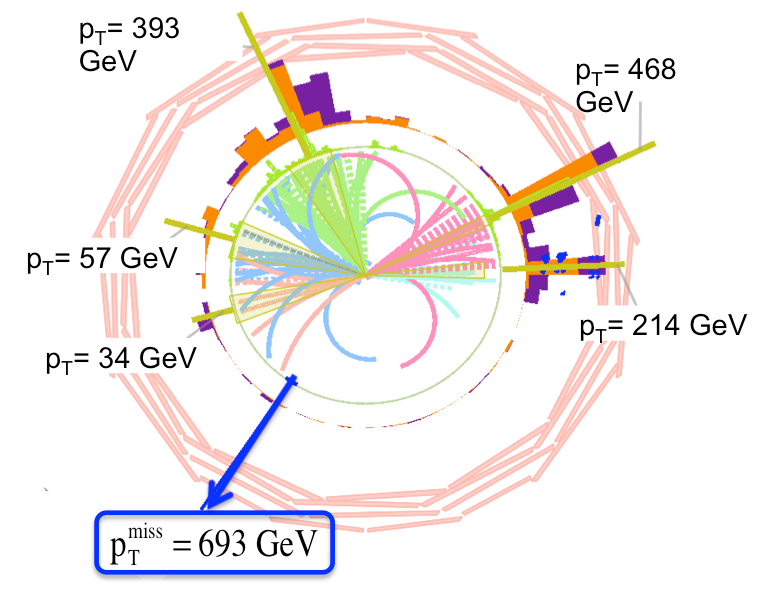
\includegraphics[height=7cm]{dmed2.png}

         \end{figure}

         \begin{itemize}
         %\color{white}
          \tiny
          \item Search for direct dark matter production in top quark pair events
         \end{itemize}
    };
   \node[insideFancytitle, left=\insideTitleOffset] at ($(nn.north east)+(0,0.5)$){\normalsize Search for dark matter}; 
    
    
       
    
    \node[insideBoxStyle, text width=\subBoxWidth, anchor=north west,minimum height=\topRowHeightRight] (majorana) at ($(subjects.north)+(1,-8)$){
       {\tiny \\}
       \hspace{0.5cm}
       \begin{minipage}{35cm}
       {\tiny
 Only a few years ago, the Nobel prize was awarded for the discovery of neutrino oscillations,
a phenomenon strongly suggesting that neutrinos are in fact massive particles. Several experiments have however constrained this mass to be extremely small, below the eV scale.
It might be conceived as unnatural that the Higgs mechanism would be responsible
for their masses as the Yukawa couplings would have to be many orders of magnitude
smaller than those of the other SM particles. By introducing heavy sterile
neutrinos, in the SM, the mass of the left-handed neutrino can be pushed down below
the eV scale while retaining a Yukawa coupling constant similar to those of other SM
particles. This is known as the see-saw mechanism.
If they exist in nature, sterile neutrinos might also be searched for in the LHC's
proton-proton collisions. $W$ bosons, which are copiously produced at the LHC, may
decay to a heavy sterile neutrino, due to it's coupling to the neutrino, and a charged
lepton. This leads to characteristic signatures, which can be efficiently distinguished
from known Standard Model processes. No discovery was made during the LHC Run I, nor with the first data from Run II, collected in 2016 at a center-of-mass energy of 13 TeV. But the increase in integrated luminosity from the 2017 and 2018 data taking, along with refined analysis techniques and the addition of new decay channels of the heavy neutrino, will allow us to expand the horizon of these searches.
}

        \begin{figure}
                  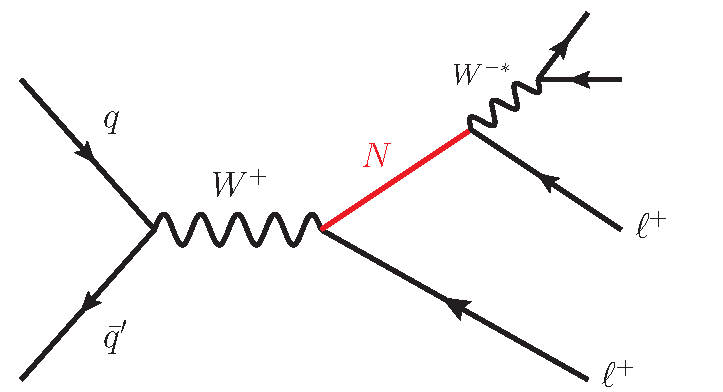
\includegraphics[height=7cm]{majoranaDiagram.pdf}
                  \hspace{3cm}
                  
\includegraphics[height=7cm]{majoranaCartoon.png}
        \end{figure}
         \begin{itemize}
        %  \color{white}
          \tiny
          \item Search for heavy sterile neutrinos in dilepton pairs + hadrons, with and without displaced vertices
          \item Search for heavy sterile neutrinos in 3 prompt lepton final states 
          \item Search for heavy sterile neutrinos in final states with hadronically decayed taus
          \item Search for heavy sterile neutrinos in B hadron decays
         \end{itemize}  

       \end{minipage}
    };
    \node[insideFancytitle, left=\insideTitleOffset] at ($(majorana.north east)+(0,0.5)$){\normalsize Searches for heavy sterile neutrinos};
    
    
   \node[insideBoxStyle, text width=\subBoxWidth, anchor=north west,minimum height=\bottomRowHeightRight] (susy) at ($(majorana.south west)+(0,-2.5)$){
       {\tiny \\}
        \hspace{0.5cm}
       \begin{minipage}{23cm}
        \tiny
        Among many theories going beyond the standard model is Supersymmetry (SUSY). It can be used to address
the problem of dark matter, and cure the hierarchy problem that afflicts the SM. SUSY is a spacetime symmetry relating fermions and bosons. In a supersymmetric theory there are an equal number of bosonic and fermionic degrees of freedom which
naturally leads to cancellations between the divergent mass corrections to the Higgs boson's mass. Every fermion would therefore have a bosonic partner in SUSY models
and vice versa. To achieve a cancellation of the chiral anomaly arising from
the fermionic partner of the Higgs, atleast one other scalar doublet is required, leading
to the presence of 5 or more scalar Higgs bosons. In order to protect
the proton from decaying, R-parity conservation is introduced, leading to the stability
of the lightest supersymmetric particle. So the requirement of a stable
proton can lead to an excellent dark matter candidate in SUSY. \\ \\
The discovery of supersymmetric particles would mark a revolutionary leap in the field
of particle physics and our understanding of nature. Several searches, approaching the
problem from different angles, are proposed.\\
        \begin{itemize}
         \tiny
     %    \color{white}
         \item Search for supersymmetry in three leptons and missing energy final states
         \item Search for supersymmetry using same-sign dileptons and missing energy
         \item Search for the stop, the supersymmetric partner of the top quark
        \end{itemize}
       \end{minipage}
       \begin{minipage}{11cm}
         \begin{figure}         
     %    \frame{\includegraphics[width=15cm]{{susylimit}.png}}
         \includegraphics[width=8cm,trim=25 25 25 25,clip]{{iceSusy}.png} \hspace{1cm} 

         \end{figure}        
       \end{minipage}
    };
    \node[insideFancytitle, left=\insideTitleOffset] at ($(susy.north east)+(0,0.5)$){\normalsize Searches for supersymmetry};
    
}